\documentclass[Modultest/Modultest_main.tex]{subfiles}
\begin{document}

\lstdefinestyle{customc}{
    breaklines=true,
    language=C,
    showstringspaces=false,
}
\lstset{style=customc}

\section{WebPage Modultest}\label{webpage_modultest}
I dette afsnit beskrives modultesten for WebPage. WebPage er et modul, som har til opgave at modtage brugerinputs i form af hold- og brugernavne samt holdfarver. Disse informationer indtastes på smartphone af brugeren, og herfra skal de behandles og videresendes til GameController klassen. For at dette er muligt, er det nødvendigt at kommunikationen mellem client og server forløber korrekt, og at WebSocket forbindelsen er pålidelig.

\subsection{Krav}
De vigtigste krav for WebPage er opsummeret i tabellen nedenfor.
\begin{table}[H]
\begin{tabular}{|l|l|l|}
\hline
ID & Krav & Prioritet \\ \hline
K2.12 & \begin{tabular}[c]{@{}l@{}}Alt tekst på WebPage skal være på sproget\\ engelsk.\end{tabular} & M \\ \hline
K2.13 & \begin{tabular}[c]{@{}l@{}}På WebPage skal der for hvert af de to hold\\ indtastes følgende \textit{\textbf{spiller oplysninger}}:\\ \textit{teamname}, \textit{username1} og \textit{username2}\end{tabular} & M \\ \hline
K2.14 & \begin{tabular}[c]{@{}l@{}}Holdnavne og brugernavne indtastet på WebPage\\ skal være tekststrenge, med en længde på mellem\\ 1 og 15 karakterer.\end{tabular} & M \\ \hline
K2.15 & \begin{tabular}[c]{@{}l@{}}På WebPage skal der for hvert af de to hold\\ kunne vælges følgende \textit{\textbf{spiller oplysninger:}}\\ \textit{holdfarve}, ved at justere intensiteten af farverne\\ rød, grøn og blå i et RGB farveskema.\end{tabular} & S \\ \hline
K2.16 & \begin{tabular}[c]{@{}l@{}}Der skal kunne vælges mindst 10 forskellige farver\\ på WebPage.\end{tabular} & S \\ \hline
K4.11 & \begin{tabular}[c]{@{}l@{}}Mindst 49 ud af 50 gange, hvor der trykkes ’Start’\\ på WebPage, skal de rigtige \textit{\textbf{spiller oplysninger}}\\ fremgå af \textit{\textbf{display}} og \textit{\textbf{Cup lights}}\end{tabular} & M \\ \hline
\end{tabular}
\caption{Krav for WebPage}
\label{tab:krav_web}
\end{table}

\subsection{Metode}
\\For at teste kravene i tabel \ref{tab:krav_web} bliver der i de følgende taget udgangspunkt i et testprogram. \textbf{K4.11} kan af gode grunde ikke testes her, men forholdene kan simuleres ved at server udskriver holdnavne, brugernavne og holdfarver i terminalen, hver gang data sendes fra client (ved tryk på 'Start'). Kravet testes altså ved at indtaste \textit{\textbf{spiller oplysninger}} på hjemmesiden og sende dem, hvorefter terminal output undersøges.
\\Når dette skal testes vil resultatet være binært, forstået på den måde, at enten sendes data korrekt til server og stemmer overens med det indtastede, eller også gør det ikke. Hvert forsøg på at sende data kan beskrives som en hændelse A med to mulige udfald: succes og fiasko.
Hvis den stokastiske variabel X beskriver antal elementer i stikprøven, med egenskaben A, kan X siges at være binomialfordelt, hvis følgende er opfyldt:\cite{binomial_wiki}
\begin{enumerate}
    \item Et forsøg udføres n gange.
    \item Hver gang forsøget udføres, registreres om en hændelse indtræffer eller ej.
    \item Udfaldene af forsøgene er uafhængige.
    \item Sandsynligheden for hændelsen A er p i alle forsøg, dvs. konstant.
\end{enumerate}
Det er imidlertid svært at forestille sig, at udfaldende af forsøgene er uafhængige. Hvis ét forsøg på at sende data fra client til server mislykkes, er der større sandsynlighed for, at
fremtidige forsøg også går galt. Man kan også forestille sig at sandsynligheden for en succesfuld overførsel aftager, jo længere WebPage tråden kører, dvs. p er ikke nødvendigvis konstant. Binomialfordelingen kan altså ikke anvendes i dette tilfælde. Der er således visse begrænsninger for, hvor meget statistik, der kan anvendes, og hvor udførlig testen kan gøres. \\
\newpage
\subsection{Fremgangsmåde og testopstilling}
Testen udføres på følgende vis:
\begin{enumerate}
    \item Kompiler programmet på host
    \item Overfør den eksekverbare fil til RPi 
    \item Afvikl ekseverbar fil på target
    \item Åbn hjemmesiden med ip-adresse 10.9.8.2 i browser
    \item Indtast holdoplysninger og tryk 'Start'
    \item Undersøg og dokumenter data sendt og modtaget
\end{enumerate}
Der foretages en stikprøve på n=50, dvs. punkterne 5 og 6 gentages 50 gange, mens navne og farver varieres. Herefter sammenlignes resultatet med kravene.
Hjemmesiden er vist i browseren Firefox er i figur \ref{fig:webpage_modultest_1} mens det resulterende terminal output kan ses i figur \ref{fig:webpage_modultest_2}.
\begin{figure}[H]
    \centering
    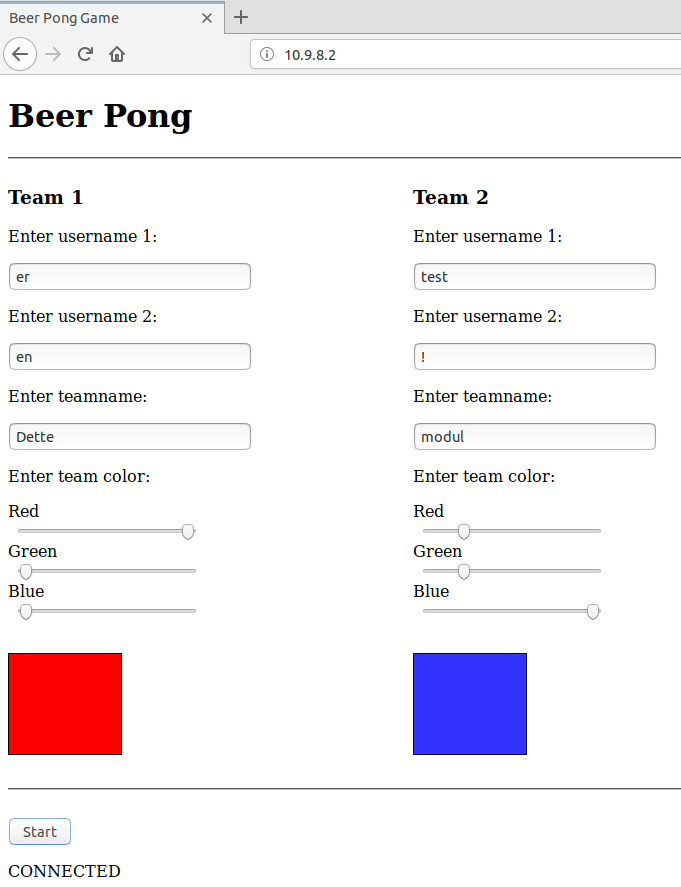
\includegraphics[width=0.6\textwidth]{Modultest/WebPage/graphics/modultest_1.png}
    \caption{Modultest - hjemmeside vist i browser}
    \label{fig:webpage_modultest_1}
\end{figure}
\begin{figure}[H]
    \centering
    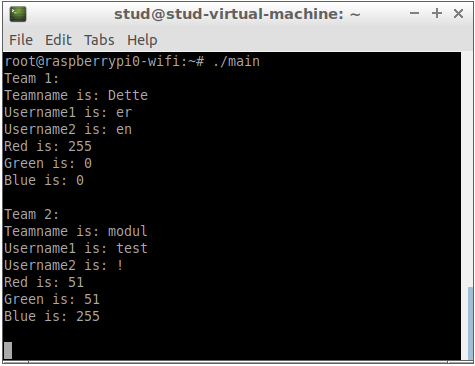
\includegraphics[width=0.7\textwidth]{Modultest/WebPage/graphics/modultest_2.png}
    \caption{Modultest - terminal output}
    \label{fig:webpage_modultest_2}
\end{figure}

\subsection{Resultater}
Resultatet af modultesten fremgår af tabel \ref{tab:webpage_data_1}. En fejl vil i dette tilfælde ske på én af tre følgende måder:
\begin{itemize}
    \item Data sendes ikke fra client men modtages af serveren (falsk positiv)
    \item Data sendes fra client med modtages ikke af serveren (falsk negativ)
    \item Data sendes fra client og modtages af serveren, men data er ikke korrekt
\end{itemize}
Som det ses nedenfor er data sendt og modtaget korrekt alle 50 gange. 
\begin{table}[H]
    \centering
    \begin{tabular}{|L{0.15\textwidth}|L{0.15\textwidth}|L{0.15\textwidth}|}
         \hline
         \textbf{Forsøg, n} & \textbf{Korrekt output} & \textbf{Fejl} \\ \hline
         50 & 50 & 0 \\ \hline 
    \end{tabular}
    \caption{Data sendes fra client til server 50 gange}
     \label{tab:webpage_data_1}
\end{table}

\subsection{Konklusion}
Kravene i tabel \ref{tab:krav_web} kræver visuel inspektion af hjemmesiden i figur \ref{fig:webpage_modultest_1}. Alt teksten er engelsk, så krav \textbf{K2.12} kan siges at være opfyldt. Det er desuden muligt at indtaste holdnavne og brugernavne, og disse kan ikke overskride en længde på 15 karakterer. Kravene \textbf{K2.13} og \textbf{K2.14} kan betragtes som værende opfyldt. Der er implementeret en løsning med tre track bars til at vælge farver. Der kan dermed vælges mellem 256 $\cdot$ 256 $\cdot$ 256 = 16.777.216 farver. Kravene \textbf{K2.15} og \textbf{K2.16} er derfor også opfyldt. \textbf{K4.11} kan dog først siges at være opfyldt efter en succesfuld accepttest, hvor WebPage er integreret med \textit{\textbf{display}} og \textit{\textbf{Cup lights}}.
\end{document}